
%% bare_conf.tex
%% V1.3
%% 2007/01/11
%% by Michael Shell
%% See:
%% http://www.michaelshell.org/
%% for current contact information.
%%
%% This is a skeleton file demonstrating the use of IEEEtran.cls
%% (requires IEEEtran.cls version 1.7 or later) with an IEEE conference paper.
%%
%% Support sites:
%% http://www.michaelshell.org/tex/ieeetran/
%% http://www.ctan.org/tex-archive/macros/latex/contrib/IEEEtran/
%% and
%% http://www.ieee.org/

%%*************************************************************************
%% Legal Notice:
%% This code is offered as-is without any warranty either expressed or
%% implied; without even the implied warranty of MERCHANTABILITY or
%% FITNESS FOR A PARTICULAR PURPOSE! 
%% User assumes all risk.
%% In no event shall IEEE or any contributor to this code be liable for
%% any damages or losses, including, but not limited to, incidental,
%% consequential, or any other damages, resulting from the use or misuse
%% of any information contained here.
%%
%% All comments are the opinions of their respective authors and are not
%% necessarily endorsed by the IEEE.
%%
%% This work is distributed under the LaTeX Project Public License (LPPL)
%% ( http://www.latex-project.org/ ) version 1.3, and may be freely used,
%% distributed and modified. A copy of the LPPL, version 1.3, is included
%% in the base LaTeX documentation of all distributions of LaTeX released
%% 2003/12/01 or later.
%% Retain all contribution notices and credits.
%% ** Modified files should be clearly indicated as such, including  **
%% ** renaming them and changing author support contact information. **
%%
%% File list of work: IEEEtran.cls, IEEEtran_HOWTO.pdf, bare_adv.tex,
%%                    bare_conf.tex, bare_jrnl.tex, bare_jrnl_compsoc.tex
%%*************************************************************************

% *** Authors should verify (and, if needed, correct) their LaTeX system  ***
% *** with the testflow diagnostic prior to trusting their LaTeX platform ***
% *** with production work. IEEE's font choices can trigger bugs that do  ***
% *** not appear when using other class files.                            ***
% The testflow support page is at:
% http://www.michaelshell.org/tex/testflow/



% Note that the a4paper option is mainly intended so that authors in
% countries using A4 can easily print to A4 and see how their papers will
% look in print - the typesetting of the document will not typically be
% affected with changes in paper size (but the bottom and side margins will).
% Use the testflow package mentioned above to verify correct handling of
% both paper sizes by the user's LaTeX system.
%
% Also note that the "draftcls" or "draftclsnofoot", not "draft", option
% should be used if it is desired that the figures are to be displayed in
% draft mode.
%
\documentclass[10pt, conference, compsocconf]{IEEEtran}
% Add the compsocconf option for Computer Society conferences.
%
% If IEEEtran.cls has not been installed into the LaTeX system files,
% manually specify the path to it like:
% \documentclass[conference]{../sty/IEEEtran}


% Add amsmath for sideset
\usepackage{amsmath}


% Some very useful LaTeX packages include:
% (uncomment the ones you want to load)


% *** MISC UTILITY PACKAGES ***
%
%\usepackage{ifpdf}
% Heiko Oberdiek's ifpdf.sty is very useful if you need conditional
% compilation based on whether the output is pdf or dvi.
% usage:
% \ifpdf
%   % pdf code
% \else
%   % dvi code
% \fi
% The latest version of ifpdf.sty can be obtained from:
% http://www.ctan.org/tex-archive/macros/latex/contrib/oberdiek/
% Also, note that IEEEtran.cls V1.7 and later provides a builtin
% \ifCLASSINFOpdf conditional that works the same way.
% When switching from latex to pdflatex and vice-versa, the compiler may
% have to be run twice to clear warning/error messages.






% *** CITATION PACKAGES ***
%
%\usepackage{cite}
% cite.sty was written by Donald Arseneau
% V1.6 and later of IEEEtran pre-defines the format of the cite.sty package
% \cite{} output to follow that of IEEE. Loading the cite package will
% result in citation numbers being automatically sorted and properly
% "compressed/ranged". e.g., [1], [9], [2], [7], [5], [6] without using
% cite.sty will become [1], [2], [5]--[7], [9] using cite.sty. cite.sty's
% \cite will automatically add leading space, if needed. Use cite.sty's
% noadjust option (cite.sty V3.8 and later) if you want to turn this off.
% cite.sty is already installed on most LaTeX systems. Be sure and use
% version 4.0 (2003-05-27) and later if using hyperref.sty. cite.sty does
% not currently provide for hyperlinked citations.
% The latest version can be obtained at:
% http://www.ctan.org/tex-archive/macros/latex/contrib/cite/
% The documentation is contained in the cite.sty file itself.






% *** GRAPHICS RELATED PACKAGES ***
%
\ifCLASSINFOpdf
  \usepackage[pdftex]{graphicx}
  % declare the path(s) where your graphic files are
  % \graphicspath{{../pdf/}{../jpeg/}}
  % and their extensions so you won't have to specify these with
  % every instance of \includegraphics
  % \DeclareGraphicsExtensions{.pdf,.jpeg,.png}
\else
  % or other class option (dvipsone, dvipdf, if not using dvips). graphicx
  % will default to the driver specified in the system graphics.cfg if no
  % driver is specified.
  \usepackage[dvips]{graphicx}
  % declare the path(s) where your graphic files are
  % \graphicspath{{../eps/}}
  % and their extensions so you won't have to specify these with
  % every instance of \includegraphics
  % \DeclareGraphicsExtensions{.eps}
\fi
% graphicx was written by David Carlisle and Sebastian Rahtz. It is
% required if you want graphics, photos, etc. graphicx.sty is already
% installed on most LaTeX systems. The latest version and documentation can
% be obtained at: 
% http://www.ctan.org/tex-archive/macros/latex/required/graphics/
% Another good source of documentation is "Using Imported Graphics in
% LaTeX2e" by Keith Reckdahl which can be found as epslatex.ps or
% epslatex.pdf at: http://www.ctan.org/tex-archive/info/
%
% latex, and pdflatex in dvi mode, support graphics in encapsulated
% postscript (.eps) format. pdflatex in pdf mode supports graphics
% in .pdf, .jpeg, .png and .mps (metapost) formats. Users should ensure
% that all non-photo figures use a vector format (.eps, .pdf, .mps) and
% not a bitmapped formats (.jpeg, .png). IEEE frowns on bitmapped formats
% which can result in "jaggedy"/blurry rendering of lines and letters as
% well as large increases in file sizes.
%
% You can find documentation about the pdfTeX application at:
% http://www.tug.org/applications/pdftex





% *** MATH PACKAGES ***
%
%\usepackage[cmex10]{amsmath}
% A popular package from the American Mathematical Society that provides
% many useful and powerful commands for dealing with mathematics. If using
% it, be sure to load this package with the cmex10 option to ensure that
% only type 1 fonts will utilized at all point sizes. Without this option,
% it is possible that some math symbols, particularly those within
% footnotes, will be rendered in bitmap form which will result in a
% document that can not be IEEE Xplore compliant!
%
% Also, note that the amsmath package sets \interdisplaylinepenalty to 10000
% thus preventing page breaks from occurring within multiline equations. Use:
%\interdisplaylinepenalty=2500
% after loading amsmath to restore such page breaks as IEEEtran.cls normally
% does. amsmath.sty is already installed on most LaTeX systems. The latest
% version and documentation can be obtained at:
% http://www.ctan.org/tex-archive/macros/latex/required/amslatex/math/



% Package for colour:
\usepackage{color}

% *** SPECIALIZED LIST PACKAGES ***
%
\usepackage{algorithm}
\usepackage{algorithmicx}
\usepackage{algpseudocode}
% algorithmic.sty was written by Peter Williams and Rogerio Brito.
% This package provides an algorithmic environment fo describing algorithms.
% You can use the algorithmic environment in-text or within a figure
% environment to provide for a floating algorithm. Do NOT use the algorithm
% floating environment provided by algorithm.sty (by the same authors) or
% algorithm2e.sty (by Christophe Fiorio) as IEEE does not use dedicated
% algorithm float types and packages that provide these will not provide
% correct IEEE style captions. The latest version and documentation of
% algorithmic.sty can be obtained at:
% http://www.ctan.org/tex-archive/macros/latex/contrib/algorithms/
% There is also a support site at:
% http://algorithms.berlios.de/index.html
% Also of interest may be the (relatively newer and more customizable)
% algorithmicx.sty package by Szasz Janos:
% http://www.ctan.org/tex-archive/macros/latex/contrib/algorithmicx/




% *** ALIGNMENT PACKAGES ***
%
%\usepackage{array}
% Frank Mittelbach's and David Carlisle's array.sty patches and improves
% the standard LaTeX2e array and tabular environments to provide better
% appearance and additional user controls. As the default LaTeX2e table
% generation code is lacking to the point of almost being broken with
% respect to the quality of the end results, all users are strongly
% advised to use an enhanced (at the very least that provided by array.sty)
% set of table tools. array.sty is already installed on most systems. The
% latest version and documentation can be obtained at:
% http://www.ctan.org/tex-archive/macros/latex/required/tools/


%\usepackage{mdwmath}
%\usepackage{mdwtab}
% Also highly recommended is Mark Wooding's extremely powerful MDW tools,
% especially mdwmath.sty and mdwtab.sty which are used to format equations
% and tables, respectively. The MDWtools set is already installed on most
% LaTeX systems. The lastest version and documentation is available at:
% http://www.ctan.org/tex-archive/macros/latex/contrib/mdwtools/


% IEEEtran contains the IEEEeqnarray family of commands that can be used to
% generate multiline equations as well as matrices, tables, etc., of high
% quality.


%\usepackage{eqparbox}
% Also of notable interest is Scott Pakin's eqparbox package for creating
% (automatically sized) equal width boxes - aka "natural width parboxes".
% Available at:
% http://www.ctan.org/tex-archive/macros/latex/contrib/eqparbox/





% *** SUBFIGURE PACKAGES ***
\usepackage[tight,footnotesize]{subfigure}
% subfigure.sty was written by Steven Douglas Cochran. This package makes it
% easy to put subfigures in your figures. e.g., "Figure 1a and 1b". For IEEE
% work, it is a good idea to load it with the tight package option to reduce
% the amount of white space around the subfigures. subfigure.sty is already
% installed on most LaTeX systems. The latest version and documentation can
% be obtained at:
% http://www.ctan.org/tex-archive/obsolete/macros/latex/contrib/subfigure/
% subfigure.sty has been superceeded by subfig.sty.



%\usepackage[caption=false]{caption}
%\usepackage[font=footnotesize]{subfig}
% subfig.sty, also written by Steven Douglas Cochran, is the modern
% replacement for subfigure.sty. However, subfig.sty requires and
% automatically loads Axel Sommerfeldt's caption.sty which will override
% IEEEtran.cls handling of captions and this will result in nonIEEE style
% figure/table captions. To prevent this problem, be sure and preload
% caption.sty with its "caption=false" package option. This is will preserve
% IEEEtran.cls handing of captions. Version 1.3 (2005/06/28) and later 
% (recommended due to many improvements over 1.2) of subfig.sty supports
% the caption=false option directly:
%\usepackage[caption=false,font=footnotesize]{subfig}
%
% The latest version and documentation can be obtained at:
% http://www.ctan.org/tex-archive/macros/latex/contrib/subfig/
% The latest version and documentation of caption.sty can be obtained at:
% http://www.ctan.org/tex-archive/macros/latex/contrib/caption/




% *** FLOAT PACKAGES ***
%
%\usepackage{fixltx2e}
% fixltx2e, the successor to the earlier fix2col.sty, was written by
% Frank Mittelbach and David Carlisle. This package corrects a few problems
% in the LaTeX2e kernel, the most notable of which is that in current
% LaTeX2e releases, the ordering of single and double column floats is not
% guaranteed to be preserved. Thus, an unpatched LaTeX2e can allow a
% single column figure to be placed prior to an earlier double column
% figure. The latest version and documentation can be found at:
% http://www.ctan.org/tex-archive/macros/latex/base/



\usepackage{stfloats}
% stfloats.sty was written by Sigitas Tolusis. This package gives LaTeX2e
% the ability to do double column floats at the bottom of the page as well
% as the top. (e.g., "\begin{figure*}[!b]" is not normally possible in
% LaTeX2e). It also provides a command:
%\fnbelowfloat
% to enable the placement of footnotes below bottom floats (the standard
% LaTeX2e kernel puts them above bottom floats). This is an invasive package
% which rewrites many portions of the LaTeX2e float routines. It may not work
% with other packages that modify the LaTeX2e float routines. The latest
% version and documentation can be obtained at:
% http://www.ctan.org/tex-archive/macros/latex/contrib/sttools/
% Documentation is contained in the stfloats.sty comments as well as in the
% presfull.pdf file. Do not use the stfloats baselinefloat ability as IEEE
% does not allow \baselineskip to stretch. Authors submitting work to the
% IEEE should note that IEEE rarely uses double column equations and
% that authors should try to avoid such use. Do not be tempted to use the
% cuted.sty or midfloat.sty packages (also by Sigitas Tolusis) as IEEE does
% not format its papers in such ways.





% *** PDF, URL AND HYPERLINK PACKAGES ***
%
%\usepackage{url}
% url.sty was written by Donald Arseneau. It provides better support for
% handling and breaking URLs. url.sty is already installed on most LaTeX
% systems. The latest version can be obtained at:
% http://www.ctan.org/tex-archive/macros/latex/contrib/misc/
% Read the url.sty source comments for usage information. Basically,
% \url{my_url_here}.





% *** Do not adjust lengths that control margins, column widths, etc. ***
% *** Do not use packages that alter fonts (such as pslatex).         ***
% There should be no need to do such things with IEEEtran.cls V1.6 and later.
% (Unless specifically asked to do so by the journal or conference you plan
% to submit to, of course. )


% correct bad hyphenation here
\hyphenation{op-tical net-works semi-conduc-tor}


\begin{document}
%
% paper title
% can use linebreaks \\ within to get better formatting as desired
\title{Optimising energy and overhead for large parameter space simulations}


% author names and affiliations
% use a multiple column layout for up to two different
% affiliations

%\author{\IEEEauthorblockN{Alex Kell, Matthew Forshaw, A. Stephen McGough}
%\IEEEauthorblockA{School of Computing\\
%Newcastle University\\
%Newcastle, UK\\
%\{a.kell2, matthew.forshaw, stephen.mcgough\}@newcastle.ac.uk}
\author{\IEEEauthorblockN{Author1, Author2, Author3}
\IEEEauthorblockA{Institution, City, Country\\
\{author1, author2, author3\}@organisation.com}
%\IEEEauthorblockN{Authors Name/s per 2nd Affiliation (Author)}
%\IEEEauthorblockA{line 1 (of Affiliation): dept. name of organization\\
%line 2: name of organization, acronyms acceptable\\
%line 3: City, Country\\
%line 4: Email: name@xyz.com}
}

% conference papers do not typically use \thanks and this command
% is locked out in conference mode. If really needed, such as for
% the acknowledgment of grants, issue a \IEEEoverridecommandlockouts
% after \documentclass

% for over three affiliations, or if they all won't fit within the width
% of the page, use this alternative format:
% 
%\author{\IEEEauthorblockN{Michael Shell\IEEEauthorrefmark{1},
%Homer Simpson\IEEEauthorrefmark{2},
%James Kirk\IEEEauthorrefmark{3}, 
%Montgomery Scott\IEEEauthorrefmark{3} and
%Eldon Tyrell\IEEEauthorrefmark{4}}
%\IEEEauthorblockA{\IEEEauthorrefmark{1}School of Electrical and Computer Engineering\\
%Georgia Institute of Technology,
%Atlanta, Georgia 30332--0250\\ Email: see http://www.michaelshell.org/contact.html}
%\IEEEauthorblockA{\IEEEauthorrefmark{2}Twentieth Century Fox, Springfield, USA\\
%Email: homer@thesimpsons.com}
%\IEEEauthorblockA{\IEEEauthorrefmark{3}Starfleet Academy, San Francisco, California 96678-2391\\
%Telephone: (800) 555--1212, Fax: (888) 555--1212}
%\IEEEauthorblockA{\IEEEauthorrefmark{4}Tyrell Inc., 123 Replicant Street, Los Angeles, California 90210--4321}}




% use for special paper notices
%\IEEEspecialpapernotice{(Invited Paper)}




% make the title area
\maketitle

%%%%%%%%%%%%%%%%%%%%%%%%%%%%%%%%%%%%%%%%%%%%%%%%%%%%%%%%%%%%%%%%%%%%%%%%%%%%%%%
\begin{abstract}
The abstract goes here. DO NOT USE SPECIAL CHARACTERS, SYMBOLS, OR MATH IN YOUR TITLE OR ABSTRACT.

\end{abstract}
%%%%%%%%%%%%%%%%%%%%%%%%%%%%%%%%%%%%%%%%%%%%%%%%%%%%%%%%%%%%%%%%%%%%%%%%%%%%%%%

\begin{IEEEkeywords}
component; formatting; style; styling;

\end{IEEEkeywords}


% For peer review papers, you can put extra information on the cover
% page as needed:
% \ifCLASSOPTIONpeerreview
% \begin{center} \bfseries EDICS Category: 3-BBND \end{center}
% \fi
%
% For peerreview papers, this IEEEtran command inserts a page break and
% creates the second title. It will be ignored for other modes.
\IEEEpeerreviewmaketitle


%%%%%%%%%%%%%%%%%%%%%%%%%%%%%%%%%%%%%%%%%%%%%%%%%%%%%%%%%%%%%%%%%%%%%%%%%%%%%%%
\section{Introduction {\color{red}Steve}}
% no \IEEEPARstart
There is a strong desire to model real-world systems through computer simulation -- a software system which replicates the salient features of the real-world system. This permits `what if' analysis, where one desires to know how the real-world system will be effected by changes in environment or policy. This is especially important when the proposed changes to the real system would be unpalatable to perform -- such as costing too much or potentially causing a degradation of service. 

In recent years the concept of the `digital twin' has emerged where the digital twin is not just a simulation based around a common type of real-world system but around one specific instance of a system. Here one can predict how changes would effect just that system. Thus allowing individual based changes of the digital twin which can then be used within the real-world system. For example optimising the parameters which control how the system would perform. Traditionally this would be very difficult to perform on the real-world system due to fears that these changes could have a detrimental impact on the performance of the system. However, by making the changes to the digital twin we remove this risk and can perform many simulations faster-than-real-time in order to identify the `optimal' set of parameters.

One may assume that to find the optimal set of parameters for a simulation, where we are optimising over a single output metric -- referred to as an objective, is just the process of running the simulation many times until the `best' set is found. Unfortunately, this is far too often not the case. The search space over which parameters can be varied and the number of possible parameters can be far larger than what can be feasibly (or sensibly) searched. One may conclude that each individual parameter may be optimised in isolation. However, if the relationship between parameters and the objective is complex then the optimal value for one parameter may not be part of the global optimal. 

This complexity can be compounded when one wishes to optimise for more than one objective -- for example the energy used by a system and the increase in time to perform the work. If one is fortunate that these outcomes are mutually constructive then this degrades to the single optimisation case. However, in most cases these multiple objectives are destructive in nature. In our example here of energy and increase of time, using only the lowest energy consuming computers can minimise energy consumption. Though at the expense of delaying work completion when the number of available low-power computers is less than the work to be completed.

In order to deal with optimising over multiple objectives to one may choose to optimise for one outcome over the other or to optimise for a combination ratio of the different outcomes. However, this removes full transparency of the interplay between optimising for the different objectives -- allowing for decisions to be made over full knowledge.

By contrast in this work we overcome the two problems of search space and multiple objectives through the use of a Genetic Algorithm~\cite{mitchell1995genetic} along with the generation of a Pareto frontier~\cite{Pareto1927, Stadler1979} through the use of the Non-Dominated Sorting Genetic Algorithm II (NSGA-II)~\cite{Valkanas2014}. The use of a Genetic Algorithm allows us to quickly identify those parameters which lead to optimal output by repeatedly selecting parameters which are mutations from previous generations. By using NSGA-II	 we are able to identify those parameter which lie along the Pareto frontier -- a curve which identifies, for each combination of objectives, those points for which there is no (yet identified\footnote{Note that as we do not try every combination of parameters it may be possible to improve these points.}) combination of parameters which would improve one of the objectives without diminishing one of the other objectives.

We exemplify this approach here for the digital twin which we can tailor from the HTC-Sim~\cite{htc-sim} simulation system of a high-throughput computing HTCondor~\cite{htcondor} setup. In the case here we wish to deploy a scheduler over the HTCondor system to optimise the selection of resources on which to run the individual tasks\footnote{Here a task is a single executable which is run on one computer within the HTCondor system.}. Our scheduler employs a Reinforcement Learning~\cite{rl} (RL) approach based on the work by McGough \textit{et al.}~\cite{suscom}. We identify twenty parameters from this work which can be used to configure the RL scheduler and consider the two objectives of energy consumed by the system and average overhead per task.
	
{\color{red}Contributions?}

The rest of this paper is set out as follows. In Section \ref{motivation} we motivate the need to perform a Genetic Algorithm along with Pareto frontier identification on the HTCondor RL scheduler. We present related work in Section \ref{relatedWork} followed by a detailed discussion of the optimisation method in Section \ref{method}. Section \ref{environment} details the environment we are simulating, while results are presented in Section \ref{results}. We offer conclusions and identify future directions in Section \ref{conc}.	

%Often we desire to optimise a system for multiple constraints -- such as energy used and the overhead seen by the users of the system in a high throughput computing system. Where overhead is defined as the time in excess of the actual execution time for running through the system. Unless we are very fortunate these multiple constraints will be mutually incompatible with each other. In our example here we can reduce the energy consumed in the high-throughput system by only using the most energy-efficient computers, however, this will reduce the number of computers available and hence increase the overhead seen by the user. This is compounded by the fact that many systems are parameterised by multiple parameters where the variation of these parameters can have unpredictable and interacting effects.
	
% You must have at least 2 lines in the paragraph with the drop letter
% (should never be an issue)

%%%%%%%%%%%%%%%%%%%%%%%%%%%%%%%%%%%%%%%%%%%%%%%%%%%%%%%%%%%%%%%%%%%%%%%%%%%%%%%
\section{Motivation{\color{red}Steve}}
\label{motivation}

Parameter spaces for simulations rapidly become large as the number of parameters and valid values for each parameter increases. This is perhaps why in their work McGough \textit{et al.}~\cite{suscom} only ever vary two input parameters at a time and even then only consider a maximum of eleven different values for each of these parameters - leading to 121 different simulations which would be executed. 

Continuous value parameters are the hardest to deal with when performing parameter space simulations. Selecting size of discretisation for the parameter is vitally important -- too small a discretisation will lead to excessively large numbers of simulations which will need running, whilst too corse a discretisation will mean one is more likely to miss the optimal value. Integer values are similar in complexity save from the fact that their is a minimum level of discretisation -- the unit value. 

Let us assume here that we wish to perform a parameter sweep over just six continuous values for a simulation which takes just five minutes per run. If we discretise each of the continuous parameters to one hundred values then we would require $10^12$ simulation runs, which is just over 9.5 million hours of simulation time. If we were to restrict the discretisation to just ten values per parameter this would reduce our parameter space to one million simulation runs and 9.5 years of simulation. Either case is far in excess of what can be performed. Thus the use of a machine learning optimisation approach is highly desirable here.

We use here Figure \ref{ohven} from \cite{suscom} to illustrate the motivation for identifying a Pareto frontier. The variation in colours represents the different learning rates of the RL approach whilst the spread of each colour represents variations in how much importance is placed on the computers selected. It can be seen from this figure that there is no global optimal -- minimising energy whilst at the same time minimising average overhead. A tradeoff needs to be made between the two objectives in terms of what has the greater significance. This figure demonstrates that a Pareto frontier is present, though, due to the small number of sample points this is most likely not the actual Pareto frontier for this problem.

\begin{figure}[t]
\centering
\includegraphics[width=0.45\textwidth]{figures/motivation/OneEta-OvE}
% where an .eps filename suffix will be assumed under latex, 
% and a .pdf suffix will be assumed for pdflatex; or what has been declared
% via \DeclareGraphicsExtensions.
\caption{Overhead and Energy compared, from \cite{suscom}}
\label{ohven}
\end{figure}


%%%%%%%%%%%%%%%%%%%%%%%%%%%%%%%%%%%%%%%%%%%%%%%%%%%%%%%%%%%%%%%%%%%%%%%%%%%%%%%
\section{Related Work{\color{red}Alex + Matt}}
\label{relatedWork}

Multi-objective optimisation problems are commonplace, with applications as diverse as electoral zone design \cite{Ponsich2017} to generation expansion planning \cite{Kannan2009}. Here we review various applications that have utilized multi-objective optimization.

Multi-objective optimization has been used in many different fields in the literature, and many multi-objective problems have been solved with the Non-Dominated Sorting Genetic Algorithm II (NSGA-II) algorithm \cite{Valkanas2014}. There are, however, examples of other algorithms being used, such as the Multi-Objective Genetic Algorithm \cite{T.MurataandH.Ishibuchi1995}.

Ponsich \textit{et al.} apply the NSGA-II algorithm to electoral zone design~\cite{Ponsich2017}. The criteria in which the geographical units must be aggregated are population equality, compactness, and contiguity. They found that the NSGA-II obtains promising results when compared with the simulated annealing algorithm, producing better-distributed solutions over a wider-spread front.

Kannan \textit{et al.} also used the NSGA-II algorithm for the generation expansion planning problem  \cite{Kannan2009}. This problem seeks to identify which generating units should be commissioned and when they should become available over the long-term planning horizon. They optimised for two trade-off solutions: to minimize cost, and minimize sum of normalized constraint violations; and to minimize investment cost and minimize outage cost. They found that they were able to find a Pareto-front with very high computational efficiency.

Wei \textit{et al.} used NSGA-II to optimize energy consumption and indoor environment thermal performance~\cite{Yu2015a}. They used simulation data which contained information on energy consumption and indoor thermal comfort. The study used a back propagation network optimised by a genetic algorithm to characterize building behaviour that was used for predicting the energy consumption and indoor thermal comfort status of residential buildings. This model was used as a fitness function to the NSGA-II algorithm.

Guha \textit{et al.} used multi-objective optimization to design a ship hull \cite{Guha2015}. As their objective functions were not smooth, they found that evolutionary techniques to attain optimum hull forms the most practical. They tested a number of different algorithms, and found that Sequential Quadratic Programming, Pattern Search and Interior-Point were very sensitive to the initial guess and prone to getting stuck in a local minima. The genetic algorithm and particle swarm optimisation, however, proved to be more robust and able to determine the global minima in most trials.

%%%%%%%%%%%%%%%%%%%%%%%%%%%%%%%%%%%%%%%%%%%%%%%%%%%%%%%%%%%%%%%%%%%%%%%%%%%%%%%
\section{Optimization methods{\color{red}Alex + Steve}}
\label{method}

Classical optimization methods, such as non-linear programming, find single solutions per simulation run. However, many real-world problems naturally have multiple objectives to optimise. Traditionally, classical optimization methods are used to optimise these multi-objective problems by artificially converting them into a single-objective problem to be solved. 

This, however, does not take into account the various trade-offs between optimal solutions, known as Pareto-optimal solutions. It, therefore, becomes important to find multiple Pareto-optimal solutions. A Pareto frontier is made up of many Pareto-optimal solutions. The results of which can be displayed graphically, enabling a user to choose between various solutions and trade-offs.

Classical methods require multiple applications of an optimization algorithm, with various scalings between rewards to achieve a single reward. The population approach of genetic algorithms, however, enable the Pareto frontier to be found in a single simulation run. An example of a multi-objective genetic algorithm is the NSGA-II, which is used in this paper.

\subsection{Genetic Algorithms}

Genetic algorithms are a class of evolutionary algorithms first proposed by John Holland in 1975 \cite{Holland1975}. We detail the workings of genetic algorithms in this section.

An initial population of individual structures $P(0)$ is generated, and each individual of the population is evaluated for fitness. A subset of individuals are chosen for mating, selected proportionally to their fitness, giving $C(t) \subset P(0)$. The better individuals are given a higher chance to reproduce and create the offspring group $C'(t)$. $C'(t)$ have characteristics dependent on the genetic operators, crossover and mutation. The genetic operators are an implementation decision \cite{FogelDavidB2009}. 

Once the new population has been created via the mutation and crossover genetic operators, the new population $P(t)$ is created by merging individuals from $C'(t)$ and $P(t-1)$. The pseudocode for this algorithm is detailed in Algorithm \ref{genetic-algorithm}.

\begin{algorithm}
\begin{algorithmic}[1]
\State $t=0$
\State initialize $P(t)$
\State evaluate structures in $P(t)$
\While {termination condition not satisfied}
\State $t=t+1$
\State select reproduction $C(t)$ from $P(t-1)$
\State recombine and mutate structures in $C(t)$

forming $C'(t)$
\State evaluate structures in $C'(t)$
\State select each individual for $P(t)$ from $C'(t)$ 

or $P(t-1)$
\EndWhile
\caption{Genetic algorithm \cite{FogelDavidB2009}}
\label{genetic-algorithm}
\end{algorithmic}
\end{algorithm}

%%%%%%
\subsection{NSGA-II}

NSGA-II is used in this work due to it being shown to be efficient for multi-objective optimization on a number of benchmark problems. It has been shown to find a better spread of solutions than The Pareto Archived Evolution Strategy (PAES) \cite{Knowles1999} and Strength Pareto EA (SPEA) \cite{Zitzler2006} when approximating the true Pareto-optimal front \cite{Valkanas2014}.

The majority of multi-objective optimization algorithms use the concept of \emph{domination} during population selection \cite{Burke2014}. Domination is the process by which two solutions of a single optimization are compared to assess whether one of the solutions dominates the other. A non-dominated genetic algorithm seeks to achieve the Pareto-optimal solution, so no single optimization solution should dominate another.

\subsubsection{Non-dominated sorting}

%The concept of domination is discussed in this section. 
We assume that there are $M$ objective functions to minimise, and that $i$ and $j$ are two solutions. In minimisation, $i<j$ denotes that solution $i$ is better than solution $j$ on a particular objective. A solution $\mathbf{x}^{(1)}$ is said to dominate the solution $\mathbf{x}^{(2)}$ if the following conditions are true:

\begin{enumerate}
  \item The solution $\mathbf{x}^{(1)}$ is no worse than $\mathbf{x}^{(2)}$ in all objectives for all $j=1,2,\ldots,M.$
  \item The solution $\mathbf{x}^{(1)}$ is better than $\mathbf{x}^{(2)}$ in at least one objective for at least one $\bar{j}\in \{ 1,2,\ldots,M\}$
\end{enumerate}


Once each of the solutions, for example $\mathbf{x}^1$ and $\mathbf{x}^2$, are calculated for the $M$ objective functions, the solutions are sorted according to their level of non-domination. An example of layering is shown in Figure \ref{fig:pareto-layering}. In this example, $f_1$ and $f_2$ are the objective functions to be minimized. The Pareto frontier is the first front which contains solutions that are not dominated by any other solution and contains the best solutions. The solutions in layer 1 are only dominated by those in the Pareto front, and are non-dominated by layer 2 and layer 3. 

The solutions are then ranked according to the level of their layer. For example, the solutions contained in the Pareto front are given a fitness rank of 1, the solutions in layer 1 are given a fitness rank of 2 and so on.

\begin{figure}[t]
  \includegraphics[width=0.45\textwidth]{figures/methods/Schematic-of-solution-layering-in-NSGA-II-algorithm-33.jpg}
  \caption{Schematic of non-dominated sorting with solution layering \cite{Ahmadi2013}}
  \label{fig:pareto-layering}
\end{figure}


\subsubsection{Density Estimation}

An average density estimation is estimated for each solution. This is done by calculating the average distance between the two points either side of the solution in question. This quantity is known as $i_{distance}$, and is an estimate of the size of the largest cuboid which contains only $i$ and no other points. 

\subsubsection{Crowded comparison operator}

Next, we use the crowded operator ($\prec_n$) to ensure that the final front is an evenly spread out Pareto-optimal front. At this stage, each of the solutions have the following two attributes:
\begin{enumerate}
  \item Non-domination rank $(i_{rank})$
  \item Local crowding distance $(i_{distance})$
\end{enumerate}

We can then define a partial order:\\
$i\prec_nj$ if $(i_{rank}<j_{rank})$ or $((i_{rank}=j_{rank})$ and $(i_{distance}>j_{distance}))$ \cite{Valkanas2014}

This order concludes that a point with a lower rank is preferred over one with a higher rank, and if two points belong to the same layer, and therefore have the same rank, the point which is located in a less dense area is preferred.


\subsubsection{Main loop}

As in the standard genetic algorithm a random population $P(0)$ is created. The population is then  sorted according to non-domination. Binary tournament selection, recombination and mutation operators are used to create a child population $C'(0)$ of size $N$. 



\begin{algorithm}
\begin{algorithmic}[1]
\State $R_t=P_t \cup C'_t$ combine parent and child population
\State $\mathcal{F} = $ fast-non-dominated-sort $(R_t)$ where $\mathcal{F}=(\mathcal{F}_1, \mathcal{F}_2,\ldots)$
\State $P_{t+1}=\emptyset$
\While $\left|P_{t+1}<N\right|$
\State crowding-distance-assignment $(\mathcal{F}_i)$ (calculate the crowding distance of $(\mathcal{F}_i)$)
\State $P_{t+1}=P_{t+1}\cup \mathcal{F}_i$
\EndWhile
\State Sort($P_{t+1}, \prec_n$) sort in descending order using $\prec_n$
\State $P_{t+1} = P_{t+1}[0:N]$ select the first $N$ elements of $P_{t+1}$
\State $Q_{t+1} = $ make-new-population$(P_{t+1})$ using selection, crossover and mutation to create the new population $Q_{t+1}$
\State $t=t+1$
\caption{NSGA-II main loop \cite{Valkanas2014}}
\label{algo:nsga2}
\end{algorithmic}
\end{algorithm}


After the first population the procedure changes. This procedure is shown in Algorithm \ref{algo:nsga2}. Initially, a combined population is formed $R(t)=P(t) \cup C'(t)$ of size $2N$. $R(t)$ is then sorted according to non-domination, producing a number of different layers based on the level of domination. A new population is now formed $(P_{t+1})$, adding solutions from each front level until the size of $P_{t+1}$ exceeds $N$. The solutions of the last accepted level are then sorted according to $\prec_n$, and a total of $N$ solutions are chosen, rejecting those from the last layer that have a smaller crowding distance \cite{Valkanas2014}.

The entire process is shown in Figure \ref{fig:nsga2-schematic}, and is repeated until the termination condition is met.

\begin{figure}
  \includegraphics[width=0.49\textwidth]{figures/methods/non-dominated-sorting}
  \caption{Schematic of the NSGA-II procedure \cite{Deb2001}.}
  \label{fig:nsga2-schematic}
\end{figure}




%%%%%%%%%%%%%%%%%%%%%%%%%%%%%%%%%%%%%%%%%%%%%%%%%%%%%%%%%%%%%%%%%%%%%%%%%%%%%%%
\section{Simulation environment{\color{red}Matt + Steve}}
\label{environment}

\subsection{HTC-Sim}
The simulation environment under consideration in this paper is HTC-Sim, a trace-driven simulation framework for energy consumption in High Throughput Computing systems~\cite{htc-sim}. This work is primarily concerned with two metrics constituting our objectives, namely average overhead and total energy consumed, described below.

\textbf{Average task overhead} is defined as the time difference between the task entering and departing the system, and the actual task execution time:% Average job overhead is defined as follows: % -- Fig. \ref{time}.
\[\frac{\sum_{j}^{t \in T} (f_{t} - q_{t} - d_{t})}{|T|}\]
\noindent for a set of tasks $T$, where $q_{t}$ and $d_{t}$ are the submission time and runtime of the task, and $f_t$ is the time the return data staging of the task finished within HTC-Sim.%  is the departure time for job $j$, and  is the runtime of job $j$.}

\textbf{Energy consumption} is the total energy consumed for the whole system. Fine-grained energy consumption results are recorded at the per- computer, cluster and system levels. Providing a breakdown of energy consumption for each state, e.g. sleep, idle, active (HTC and/or interactive user). The total energy consumption is then calculated as follows:

\begin{equation}
\sideset{}{^n_{c=0}}\sum \sideset{}{^m_{p=0}}\sum t_{c,p} E_{c,p}
\end{equation}

\noindent where $n$ is the number of computers, $m$ is the number of power states, $t_{c,p}$ is the time spent by computer $c$ in state $p$ and $E_{c,p}$ is the power consumption rate of computer $c$ in state $p$.
% TODO remove end}
%{Here we evaluate the energy consumed by the system. For HTC jobs this includes energy consumed for productive jobs -- which complete execution on a computer -- and unproductive jobs -- where jobs are evicted or the job is terminated by the HTC user or the system administrator. By also including the energy incurred through data transfer we compute the total energy impact on the system from running a HTC system. We compute the HTC energy impact as:



%{\color{red}Couple of paragraphs on what HTC-Sim is

%Need to explain what is meant by total energy consumed and average overhead}

\subsection{Reinforcement Learning Scheduler}

Reinforcement Learning~\cite{rl} is a machine learning technique used to learn how to react to an environment. In RL there is an environment which is observed by an agent. Often the agent will build a state space representing the environment. For each state in the state space is a corresponding action vector representing every action which can be taken in that state. Initially each action in the action vector has the same probability of being selected. When the agent observes the environment being in a specific state it chooses an action from the action vector based on either an explorative or exploitative policy. If an explorative policy is chosen then the action is selected at random from the action vector whilst if an exploitative policy is in force then the action which has seen the `best' historical reward is selected. The choice of policy is made by randomly selecting explorative with probability $\epsilon$ and exploitative otherwise. Once the action is completed and it is known if the action was good or bad then the action within the action vector is updated -- increasing the value if the choice was good and decreasing it otherwise.

The RL scheduler by McGough {\em et al.}~\cite{suscom} is based upon this RL approach where the state of the environment is a combination of whether computers with the HTC system are free for use and the hour of the day. The granularity of state space can be varied in size from representing each computer individually through only being aware of how many computers are free in a given cluster to only knowing how many free computers there are across the whole HTC setup. Likewise the hour of the day could be for any day (24 states) or for each hour within a week (168 states). The actions can be which computer / cluster or just the whole system to place the task on or that the task is unlikely to complete and should be held in a queue.			

%{\color{red}Couple of paragraphs on the RL scheduler in HTC-Sim}

\subsection{State space parameters}
We present here the state space parameters that the GA will search over in order to identify the optimal policies. Further details can be found in ~\cite{suscom}:

{\color{red}Bring $\epsilon$ out of the list (as common to many) and then for each explain how they could benefit energy / overhead.}

\begin{itemize}
	\item {\bf Week}: is the state space for the RL in terms of a day or a week {\em \{boolean\}}.
	\item {\bf Entity level}: is the state space for the RL in terms of individual computers, clusters of computers or just the whole system {\em (computer, cluster, whole)}.
	\item {\bf $\epsilon$ policy}: What is the $\epsilon$-greedy policy changed on? {\em \{days, previous, ratio, hit\}}. Note that this has an impact on the meaning of days, change, threshold and previousPolicy.
	\item {\bf ranges}: The date range on which to change $\epsilon$. {\em \{[0,999999], ...\}}\footnote{Although this can be an arbitrarily long list we limit this to three values for this work.},\footnote{Note $value_i \leq value_2$}.
	\item {\bf reward boundaries}: reward values over which the $\epsilon$ value will be changed. {\em \{(0,1], ...\}}$^3$,$^4$
	\item {\bf $\epsilon$}: The set of $\epsilon$ values. {\em \{(0,1], ...\}}$^3$,$^4$
	\item {\bf $\sigma$}: The amount of influence the computer energy efficiency has on RL reward {\em [0,1]}.
	\item {\bf days}: Change $\epsilon$ based on the number of days of RL which have been performed {\em [0, 365], 0 = don't use.}
	\item {\bf $\delta$}: Increase $\epsilon$ by $\delta$ if current day into RL	$\leq$ days {\em [0,1]}.
	\item {\bf history}: The number of previous tasks to consider when computing the action {\em [-1,999		999], -1 = all tasks}.
	\item {\bf gaussian}: Do we apply a gaussian decay over the task history when computing the action? {\em boolean}.
	\item {\bf prior}: If all prior actions gave a negative reward then increase $\epsilon$ by 0.1 {\em boolean}.
	\item {\bf threshold}: If the ratio of best reward to average reward is less than threshold, use the previous value of $\epsilon$ {\em [0,1]}.
	\item {\bf sanity}: Defer running a task during the same hour that the computer is due to be rebooted {\em boolean}.
\end{itemize}
                                                                
If we assume here, conservatively, that each continuous parameter is discretised into one hundred values then this creates a search space of some $2.81 x 10^{37}$. Again, assuming that the simulation takes five minutes to run for each parameter combination this is $2.67 x 10^{32}$ years.

%%%%%%%%%%%%%%%%%%%%%%%%%%%%%%%%%%%%%%%%%%%%%%%%%%%%%%%%%%%%%%%%%%%%%%%%%%%%%%%
\section{Results{\color{red}Alex + Matt + Steve}}

We first evaluate if the NSGA-II approach will lead to a Pareto frontier for total energy consumed and average overhead. Figure \ref{fig:pareto} illustrates progressive iterations of the NSGA-II algorithm with successive iterations in lighter colours. The initial (dark) colours are scattered widely whilst the final iteration (light) indicates a sharp edge closest to the two axis. It is interesting to note that although there is no global optimal for both energy and overhead the Pareto front is `sharp' in the bottom left corner indicating that there is a good compromise for both objectives. There is also a separate region of points with lower energy consumption but substantially higher overheads. This appears to be cases where tasks are only allowed to run on a small number of energy efficient resources -- at the expense of significantly reducing throughput. For all parameter sets along the Pareto front {\em sanity} was true, demonstrating that not running tasks during the hour when a computer will be rebooted was the best policy. We therefore consider {\em sanity} no further.

Table \ref{tab:optimal} presents the parameter sets and objective values for minimum overhead, minimum energy and optimal combination of speed and consumption. The optimal combination of speed and consumption was attained by first scaling average overhead and total power consumed between 0 and 100. Next, we summed the scaled overhead and total power consumed and chose the combination with the minimum value. This enabled us to choose the minimum combination of both objectives with equal weighting. The scaling, however, could be changed to suit individual preferences of power consumption or average overhead. As the following parameters were identical for all cases, we present them here rather than in the table: $\epsilon$-policy was previous, gaussian was false, $ranges_1$ was 0, ratio was 0.9375 and $R_1$ was -0.5842. The energy consumption here is far better than those presented in the paper by McGough {\em et al.}~\cite{suscom} we achieve approximately the same energy consumption as they did for their best energy case for our best overhead case and we have reduced the energy consumption for the best energy case by ~19MWh -- though at the expense of significantly increasing overhead. In comparison our compromise case outperforms the original work on both energy and overhead. It should be noted, however, that this was achieved solely through the tuning of the simulation parameters with the use of NSGA-II, as both sets of results run the same underlying code.

\begin{table*}[tb]
\caption{Parameters for optimal objectives}
\label{tab:optimal}
\begin{tabular}{r|cccccccccccccccc}
&&			\multicolumn{2}{c}{State space}\\	
type & \rotatebox{90}{change} & \rotatebox{90}{Space} & \rotatebox{90}{week} & \rotatebox{90}{days} & $\epsilon_1$ & $\epsilon_2$ & \rotatebox{90}{history} & \rotatebox{90}{prior} & \rotatebox{90}{$Ranges_2$} & $R_2$ & $R_3$ & \rotatebox{90}{threshold} & \rotatebox{90}{Energy} & \rotatebox{90}{Overhead}		 \\ \hline
Overhead & 0.9025 & Cl & F & 218 & 0.8323 & 0.3897 & 488962 & F & 0 & 0 & 0.7290 & 0.4168 & 66.64 & 10.94 \\
Energy & 0.9025 & Wh & T & 218 & 0.5496 & 0.5496 & 805676 & T & 633334 & -0.4638 & -0.4638 & 0 & 41.56 & 3864 \\
Balance & 0 & Cl & F & 0 & 0.8323 & 0.3897 & 847384 & F & 0 & -0.4638 & -0.4638 & 0.4168 & 49.26 & 22.93 \\
\end{tabular}
\end{table*}


To better understand the parameters which effect the Pareto Front, we fit a Lasso regression \cite{Tibshirani1996} to distinct clusters of the Pareto Front. Lasso regression is a linear regression technique which produces coefficients of exactly 0 to give interpretable models like subset selection. The parameters were all scaled between 1 and 100 so the coefficients could be directly compared between each parameter.

Initially, we clustered the data using the unsupervised learning technique DBSCAN \cite{Ester1996}. This technique was chosen due to its effectiveness at clustering data points which are close together. This yields better results, for our dataset, than a method such as k-means clustering which partitions the data into Voronoi cells. 
The results, shown in Figure \ref{fig:clustering}, show a large negative coefficient for ratio, epsilon 3 and reward boundaries when predicting average overhead.

The coefficients for total power show that at low average overheads, and high total power consumed, ratio, history, epsilon 1 and a false value for prior have a positive effect on increasing power consumed or reducing average overhead. That is, an increase in history leads to an increase in total power consumed.






\begin{figure*}[!b]
%\centering
%\begin{subfigure}{}
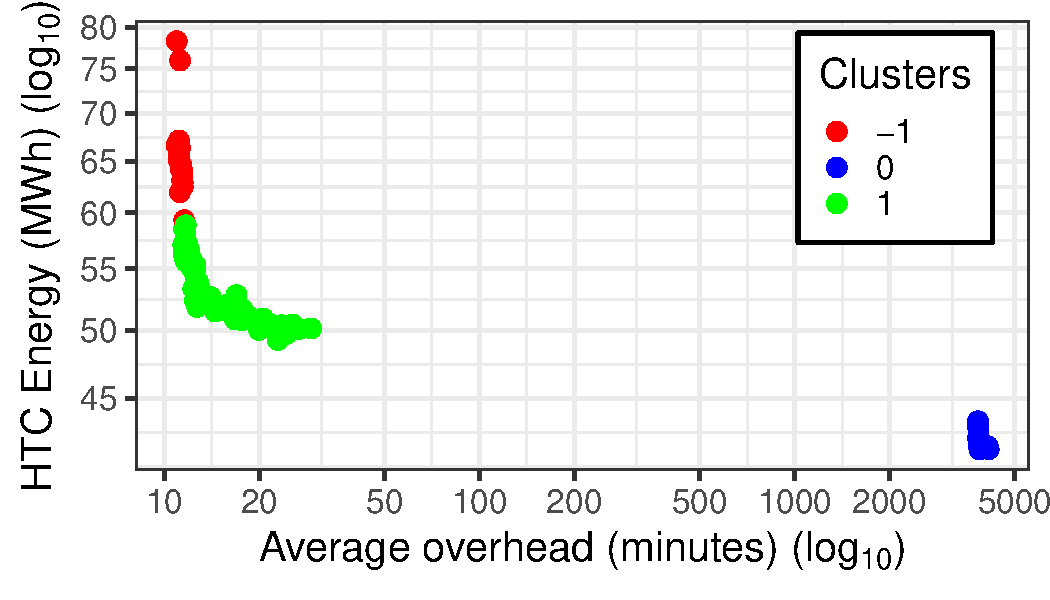
\includegraphics[width=0.3\linewidth]{figures/results/final-versions/clusters.png}%
\hfil
%\end{subfigure}
%
%\begin{subfigure}{}
\includegraphics[width=0.3\linewidth]{figures/results/final-versions/lasso_overhead.png}%
\hfil
%\end{subfigure}
%
%\begin{subfigure}{}
\includegraphics[width=0.3\linewidth]{figures/results/final-versions/lasso_power}%	
%\end{subfigure}
\caption{Objective clustering}
\label{fig:clustering}	
\end{figure*}

\begin{figure}[H]
  \includegraphics[width=0.9\linewidth]{figures/results/final-versions/all_runs_plot.png}
  \label{fig:pareto}
  \caption{Progress towards the Pareto Frontier}
\end{figure}
Figure \ref{fig:changes} demonstrates the impact of adding $\delta$ to $\epsilon$ if the RL trainer has been running for less than the prescribed number of days. Here the GA has learnt to use large values of $\delta$ when energy consumption is more important, suggesting a more explorative approach favours energy efficiency -- perhaps due to the fact that over the simulation period the state varies significantly. By contrast, the number of days shows no clear pattern. Though as the $\delta$ value is often very small this may have little if any impact.
\begin{figure}[H]
%\centering{
%\begin{subfigure}{}
%
 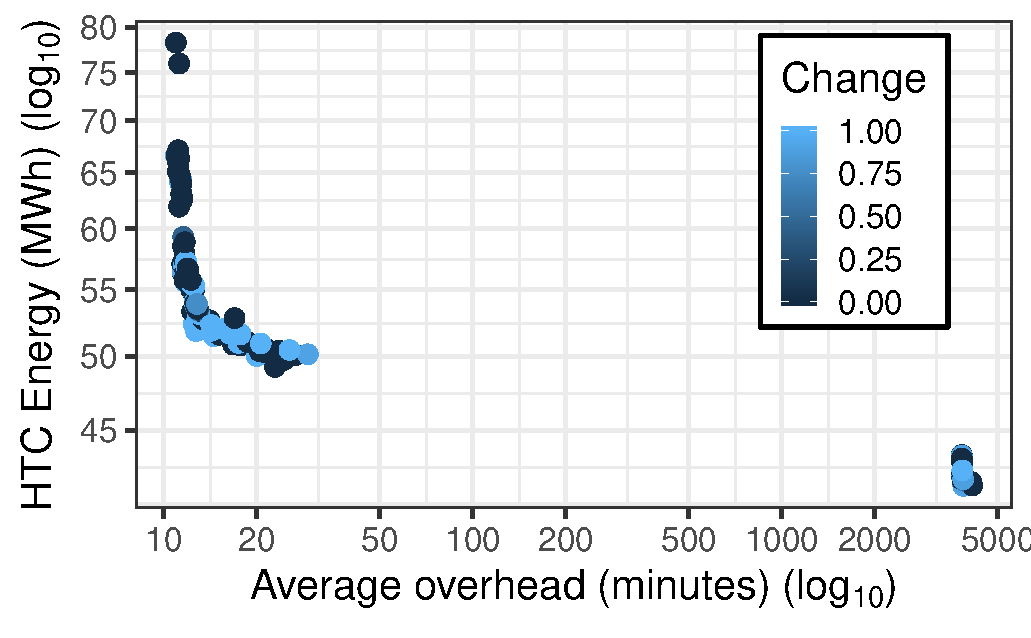
\includegraphics[width=0.45\linewidth]{figures/results/final-versions/change-avg_overhead-total_power}%
\hfil%
%\end{subfigure}
%\begin{subfigure}
%
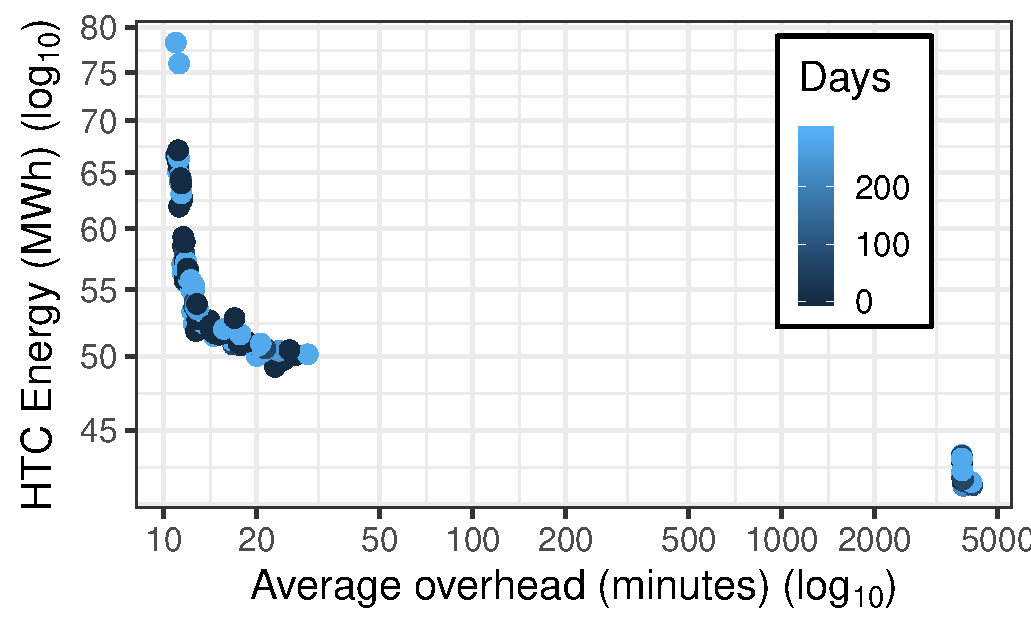
\includegraphics[width=0.45\linewidth]{figures/results/final-versions/days-avg_overhead-total_power}%
%\end{subfigure}
%
\caption{$\delta$ value and days impact on $\epsilon$}
\label{fig:changes}
\end{figure}
%\begin{figure}[H]
%	\subfloat[a) $\delta$]{\label{fig:change:delta}\includegraphics[width=60mm]{figures/results/change-power-overhead.png}}
%  \includegraphics[width=0.9\linewidth]{figures/results/change-power-overhead.png}
%  \label{fig:change}
%  \caption{$\delta$ value and days impact on $\epsilon$}
%\end{figure}
The granularity for the RL state space with respect to computers is presented in Figure \ref{fig:granularity}. Here in almost all cases the cluster level is identified as the best choice. This is most likely a consequence of the fact that it is a compromise between fine-grained computer level and course-grained whole system level. Interestingly for minimum energy whole system becomes more optimal. {\color{green} Perhaps a consequence of most tasks being held not to be executed thus the cluster not being relevant anymore.}

The other aspect of state space -- day or week -- is presented in Figure \ref{fig:week}. Here all but the most extremely long overhead cases are optimal with the day case. This would suggest that, although there is a difference based on the day of the week, this can only be exploited in the case where energy reduction is key.
\begin{figure}[H]
  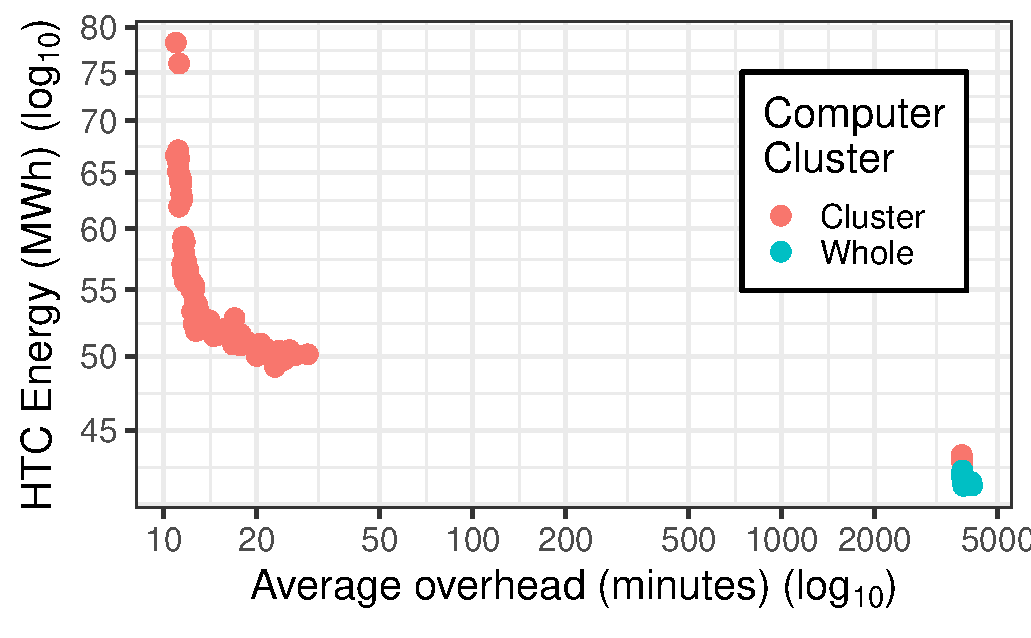
\includegraphics[width=0.9\linewidth]{figures/results/final-versions/computerClusterWhole-avg_overhead-total_power}
  \caption{Computer granularity for state space}
  \label{fig:granularity}


\end{figure}
\begin{figure}[H]
  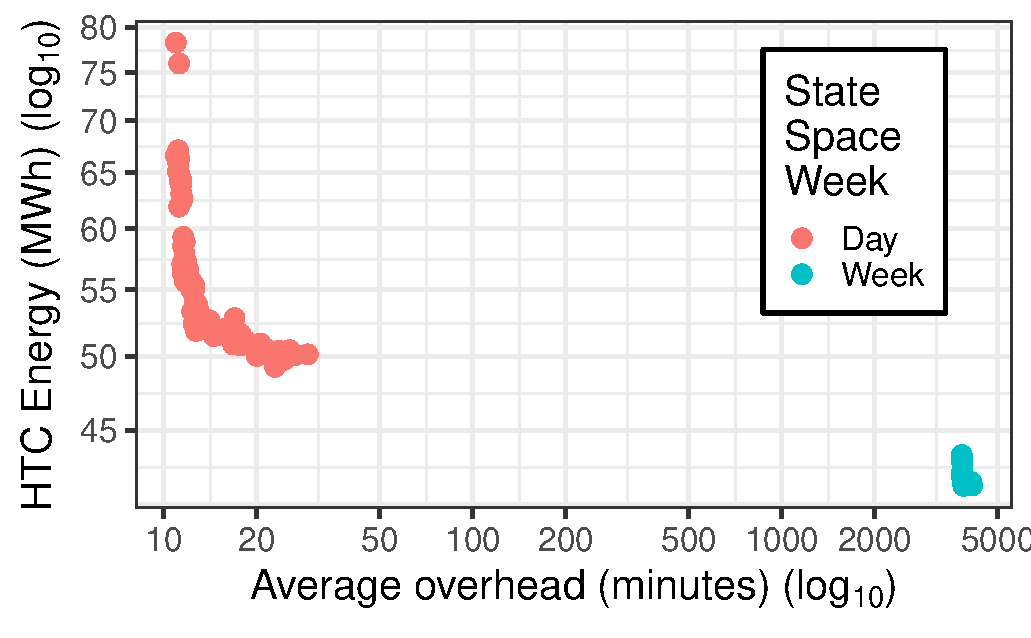
\includegraphics[width=0.9\linewidth]{figures/results/final-versions/week-avg_overhead-total_power}
  \caption{Day / Week granularity for state space}
  \label{fig:week}
\end{figure}
%
%Sanity was true in all cases.
%
%\begin{figure}[H]\includegraphics[width=0.9\linewidth]{figures/results/days-power-overhead.png}\end{figure}
%\begin{figure}[H]\includegraphics[width=0.9\linewidth]{figures/results/days-violin.png}\end{figure}
%\begin{figure}[H]\includegraphics[width=0.9\linewidth]{figures/results/epsilon-overhead-power-side-by-side.png}\end{figure}
The $\epsilon$ policy is compared in Figure \ref{fig:policy}. In almost all cases the previous policy is optimal apart from a small number of cases. This indicates that basing $\epsilon$ on the average reward of the previous day is the best policy. The ratio of best reward to average reward makes up most of the remaining points indicating that for both of these cases an adaptive policy which can move between explorative and exploitative as time moves on is the best approach -- a consequence of the state of the system changing as time progresses. Only one `static' policy is seen as optimal - where the value of $\epsilon$ changes by the number of days the RL has been running for.
\begin{figure}[H]
  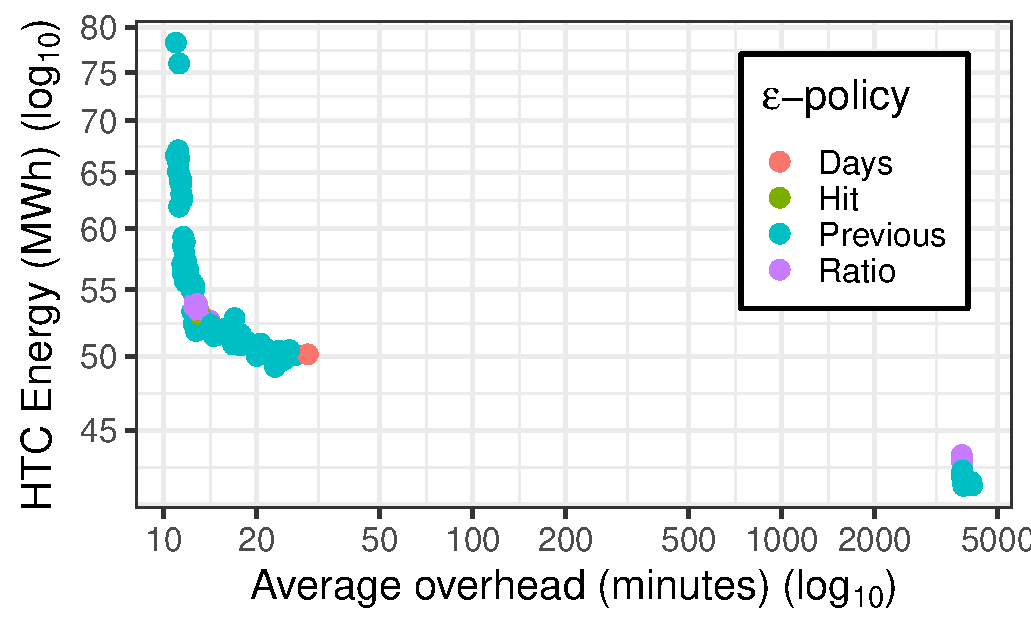
\includegraphics[width=0.9\linewidth]{figures/results/final-versions/epsilonPolicy-avg_overhead-total_power}
  \caption{$\epsilon$ policy}
  \label{fig:policy}
\end{figure}

The reward history and whether we apply a gaussian decay over this is presented in Figures \ref{fig:history} and \ref{fig:gaussian}. The size of the history seems to be bimodal with the extreme and larger overhead objectives having a value around 840,000 whilst most of the low overhead values are in the region of 500,000. Suggesting that forgetting history more quickly favours lower overheads -- but at the expense of higher energy consumption. {\color{green}By contrast the choice of when to use a gaussian decay is less obvious suggesting that other factors are at play.} 


%
\begin{figure}[H]
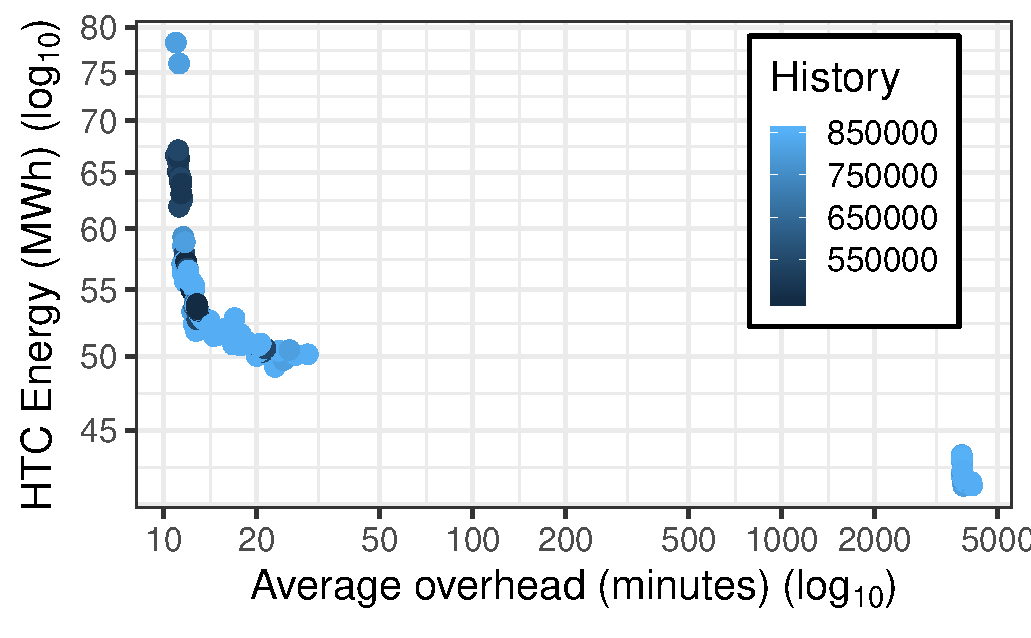
\includegraphics[width=0.9\linewidth]{figures/results/final-versions/history-avg_overhead-total_power}
  \caption{How much of the reward history is taken into account}
  \label{fig:history}
\end{figure}
%
\begin{figure}[H]
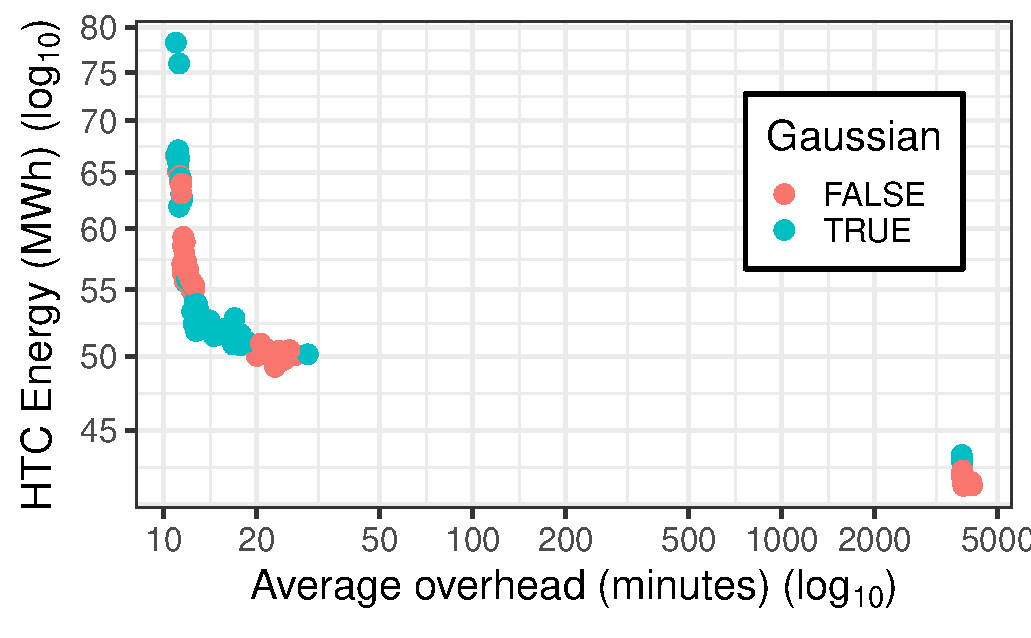
\includegraphics[width=0.9\linewidth]{figures/results/final-versions/gaussian-avg_overhead-total_power}
  \caption{Is a gaussian decay applied to the reward history}
  \label{fig:gaussian}
\end{figure}
%
%\begin{figure}[H]\includegraphics[width=0.9\linewidth]{figures/results/history-violin.png}\end{figure}
%\begin{figure}[H]\includegraphics[width=0.9\linewidth]{figures/results/iterations-overhead-total-power-log-3d.png}\end{figure}
\begin{figure}[H]\includegraphics[width=0.9\linewidth]{figures/results/final-versions/low-variables-violin}\end{figure}
%\begin{figure}[H]\includegraphics[width=0.9\linewidth]{figures/results/num-iter-average-overhead-power-condor-3d-extrme.png}\end{figure}
%\begin{figure}[H]\includegraphics[width=0.9\linewidth]{figures/results/num-iter-power-condor-low-average-overhead-3d.png}\end{figure}
\begin{figure}[H]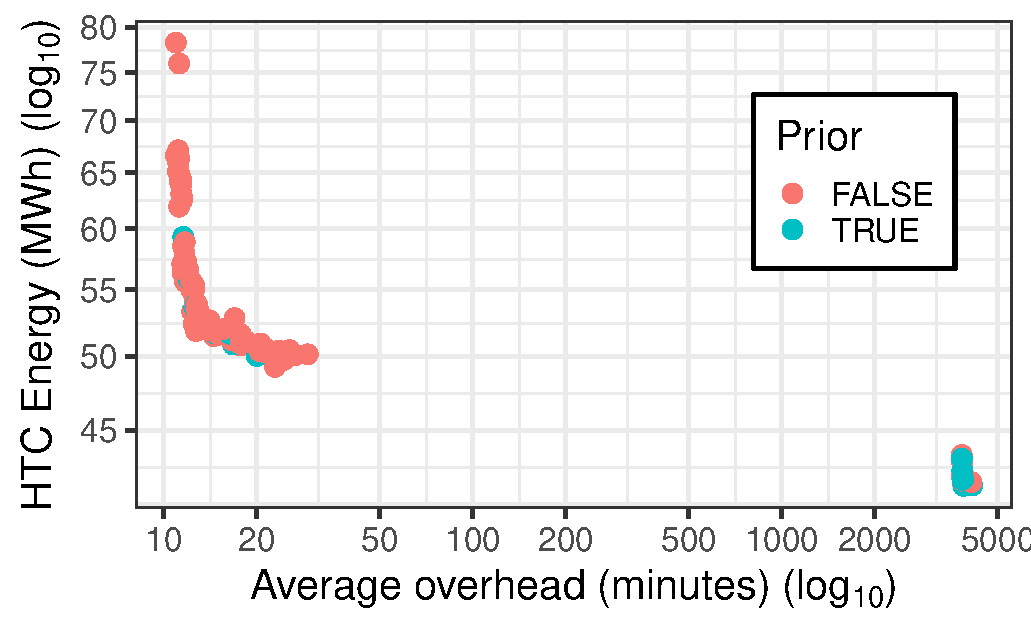
\includegraphics[width=0.9\linewidth]{figures/results/final-versions/prior-avg_overhead-total_power}\end{figure}
%\begin{figure}[H]\includegraphics[width=0.9\linewidth]{figures/results/ranges-overhead-power-side-by-side.png}\end{figure}
%\begin{figure}[H]\includegraphics[width=0.9\linewidth]{figures/results/ranges-violin.png}\end{figure}
\begin{figure}[H]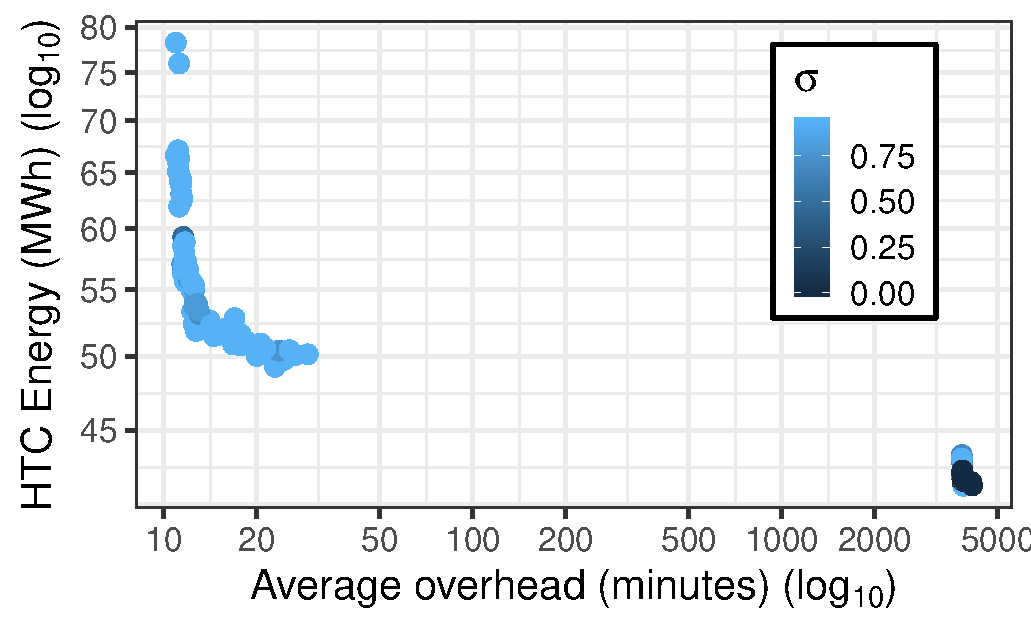
\includegraphics[width=0.9\linewidth]{figures/results/final-versions/ratio-avg_overhead-total_power}\end{figure}
%\begin{figure}[H]\includegraphics[width=0.9\linewidth]{figures/results/reward-overhead-power-side-by-side.png}\end{figure}

\begin{figure}[H]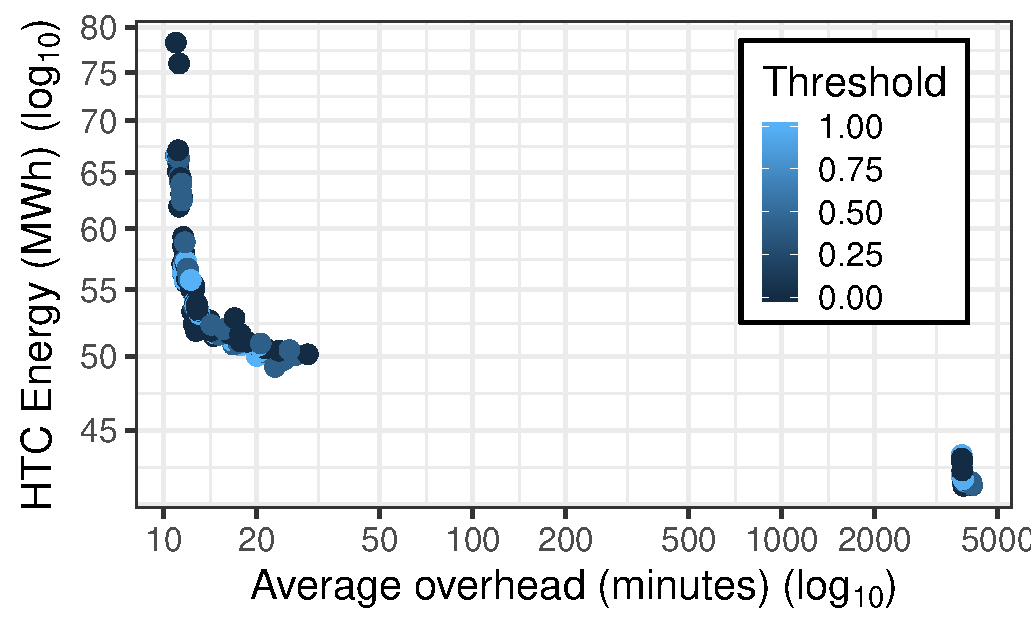
\includegraphics[width=0.9\linewidth]{figures/results/final-versions/threshold-avg_overhead-total_power}\end{figure}



\label{results}

%\section{Type style and Fonts}
%Wherever Times is specified, Times Roman or Times New Roman may be used. If neither is available on your system, please use the font closest in appearance to Times. Avoid using bit-mapped fonts if possible. True-Type 1 or Open Type fonts are preferred. Please embed symbol fonts, as well, for math, etc.


% An example of a floating figure using the graphicx package.
% Note that \label must occur AFTER (or within) \caption.
% For figures, \caption should occur after the \includegraphics.
% Note that IEEEtran v1.7 and later has special internal code that
% is designed to preserve the operation of \label within \caption
% even when the captionsoff option is in effect. However, because
% of issues like this, it may be the safest practice to put all your
% \label just after \caption rather than within \caption{}.
%
% Reminder: the "draftcls" or "draftclsnofoot", not "draft", class
% option should be used if it is desired that the figures are to be
% displayed while in draft mode.
%
%\begin{figure}[!t]
%\centering
%\includegraphics[width=2.5in]{myfigure}
% where an .eps filename suffix will be assumed under latex, 
% and a .pdf suffix will be assumed for pdflatex; or what has been declared
% via \DeclareGraphicsExtensions.
%\caption{Simulation Results}
%\label{fig_sim}
%\end{figure}

% Note that IEEE typically puts floats only at the top, even when this
% results in a large percentage of a column being occupied by floats.


% An example of a double column floating figure using two subfigures.
% (The subfig.sty package must be loaded for this to work.)
% The subfigure \label commands are set within each subfloat command, the
% \label for the overall figure must come after \caption.
% \hfil must be used as a separator to get equal spacing.
% The subfigure.sty package works much the same way, except \subfigure is
% used instead of \subfloat.
%
%\begin{figure*}[!t]
%\centerline{\subfloat[Case I]\includegraphics[width=2.5in]{subfigcase1}%
%\label{fig_first_case}}
%\hfil
%\subfloat[Case II]{\includegraphics[width=2.5in]{subfigcase2}%
%\label{fig_second_case}}}
%\caption{Simulation results}
%\label{fig_sim}
%\end{figure*}
%
% Note that often IEEE papers with subfigures do not employ subfigure
% captions (using the optional argument to \subfloat), but instead will
% reference/describe all of them (a), (b), etc., within the main caption.


% An example of a floating table. Note that, for IEEE style tables, the 
% \caption command should come BEFORE the table. Table text will default to
% \footnotesize as IEEE normally uses this smaller font for tables.
% The \label must come after \caption as always.
%
%\begin{table}[!t]
%% increase table row spacing, adjust to taste
%\renewcommand{\arraystretch}{1.3}
% if using array.sty, it might be a good idea to tweak the value of
% \extrarowheight as needed to properly center the text within the cells
%\caption{An Example of a Table}
%\label{table_example}
%\centering
%% Some packages, such as MDW tools, offer better commands for making tables
%% than the plain LaTeX2e tabular which is used here.
%\begin{tabular}{|c||c|}
%\hline
%One & Two\\
%\hline
%Three & Four\\
%\hline
%\end{tabular}
%\end{table}


% Note that IEEE does not put floats in the very first column - or typically
% anywhere on the first page for that matter. Also, in-text middle ("here")
% positioning is not used. Most IEEE journals/conferences use top floats
% exclusively. Note that, LaTeX2e, unlike IEEE journals/conferences, places
% footnotes above bottom floats. This can be corrected via the \fnbelowfloat
% command of the stfloats package.

%%%%%%%%%%%%%%%%%%%%%%%%%%%%%%%%%%%%%%%%%%%%%%%%%%%%%%%%%%%%%%%%%%%%%%%%%%%%%%%
\section{Conclusions{\color{red}Alex + Matt + Steve}}
\label{conc}
The conclusion goes here. this is more of the conclusion


%%%%%%%%%%%%%%%%%%%%%%%%%%%%%%%%%%%%%%%%%%%%%%%%%%%%%%%%%%%%%%%%%%%%%%%%%%%%%%%

% conference papers do not normally have an appendix


% use section* for acknowledgement
%\section*{Acknowledgment}


%The authors would like to thank...
%smore thanks here


% trigger a \newpage just before the given reference
% number - used to balance the columns on the last page
% adjust value as needed - may need to be readjusted if
% the document is modified later
%\IEEEtriggeratref{8}
% The "triggered" command can be changed if desired:
%\IEEEtriggercmd{\enlargethispage{-5in}}

% references section

% can use a bibliography generated by BibTeX as a .bbl file
% BibTeX documentation can be easily obtained at:
% http://www.ctan.org/tex-archive/biblio/bibtex/contrib/doc/
% The IEEEtran BibTeX style support page is at:
% http://www.michaelshell.org/tex/ieeetran/bibtex/
\bibliographystyle{IEEEtran}
% argument is your BibTeX string definitions and bibliography database(s)
%\bibliography{IEEEabrv,../bib/paper}
%
% <OR> manually copy in the resultant .bbl file
% set second argument of \begin to the number of references
% (used to reserve space for the reference number labels box)

\bibliography{bibliography,../../bib/us,../../bib/AI}



%\begin{thebibliography}{1}
%
%
%\bibitem{IEEEhowto:kopka}
%H.~Kopka and P.~W. Daly, \emph{A Guide to \LaTeX}, 3rd~ed.\hskip 1em plus
%  0.5em minus 0.4em\relax Harlow, England: Addison-Wesley, 1999.
%
%\end{thebibliography}




% that's all folks
\end{document}


